\documentclass[12pt,english]{article}
\usepackage[a4paper,bindingoffset=0.2in,%
            left=1in,right=1in,top=1in,bottom=1in,%
            footskip=.25in]{geometry}
\usepackage{blindtext}

\usepackage[english]{babel}
\usepackage[utf8]{inputenc}
\usepackage{amsmath}
\usepackage[colorinlistoftodos]{todonotes}
\usepackage{graphicx}
\usepackage{amssymb}
\usepackage[backend=bibtex]{biblatex}
\addbibresource{mybib.bib}
\usepackage[hidelinks]{hyperref}
\usepackage[title]{appendix}
\usepackage{changepage}
\usepackage{float}


\title{Correlation between Professional Domain and Facial Features based on Face Clustering}

\author{Bithiah Yuan}

\date{\today}

\begin{document}

\maketitle

%\begin{abstract}
%Bitcoin as an electronic payment system prevents the double-spending problem using the Proof-of-Work confirmation protocol. However, security issues arise with fast payments using Bitcoin as merchants are required to exchange their goods in a short time. We examine double-spending attacks on fast-payments and show how the attacks can be executed. Moreover, we demonstrate how the countermeasures by Bitcoin developers are either ineffective or produce additional costs for the merchants. Ultimately, we present an easy and lightweight solution for the dection of double-spending attacks in fast payments.


%\end{abstract}

\section{Introduction}
\label{sec:introduction}

\quad 
A significant source of information and attributes can be derived from the human face by non-verbal communication \cite{joo}. As a result, facial features have been studied extensively in the social-science domain to predict success in reaching reputable leadership positions. In particular, studies have shown that certain facial features contribute to higher salaries and more prestigious employments for CEOs. In application, the relationship between facial characteristics and social attributes can provide an more powerful objective indicator for organizations to idenity and select effective leaders within their domain than broad facial cues such as attractiveness and competence. Results have shown that a human judge can identify business, military, and sports leaders from their faces with above-chance accuracy. However, these results are biased and do not imply the actual leadership qualities of a person \cite{olivola}.

Caused by behaviour experiments from human judgement, the the research of the social attributes and facial features in the social-sciences are limited in scalability, consistency, and generalization. For example, prior familiarity to the faces of the study and personal preferences can affect the results. Therefore, a growing number of social trait judgment studies have been extended and refined to computer vision and machine learning research due to the capability of using massive datasets and large-scale processing capacity \cite{joo}.

Through a computational framework, \cite{joo} examined the relationship between facial traits and the social construction of leadership by a trained model that can predict the outcomes of political elections based on the perceived social attributes of a person's appearance. The results indicate that similar methods can be used to predict behavior in a broad range of human social relations, such as mate selection, job placement,and political and commercial negotiations \cite{joo}.

Clustering analysis is an unsupervised learning technique that groups data points into clusters based on their similarities. It is useful in grouping a collection of unlabeled data with similar nature into clusters. \cite{shi} investigated clustering a large number of unlabeled face images into individual identities present in the data \cite{shi}. The workflow shown in Figure\ref{fig:face}. consists of obtaining face representations of a collection of unlabeled data by a deep neural network. The choice of clustering algorithm then groups the face images according to their identity.

Motivated by the researches in computational social trait judgment and \cite{shi}, the following paper aims to examine the correlation between a person's profession based on their facial features through clustering face images. The clustering problem consists of the face representation and similarity metric of the face images and the choice of clustering algorithm \cite{shi}. Due to the importance of the underlying face representation in face clustering, this paper further compares different open-source state-of-the-art feature extraction methods based on deep learning.\\

\begin{figure}[!tbp]
 \centering
    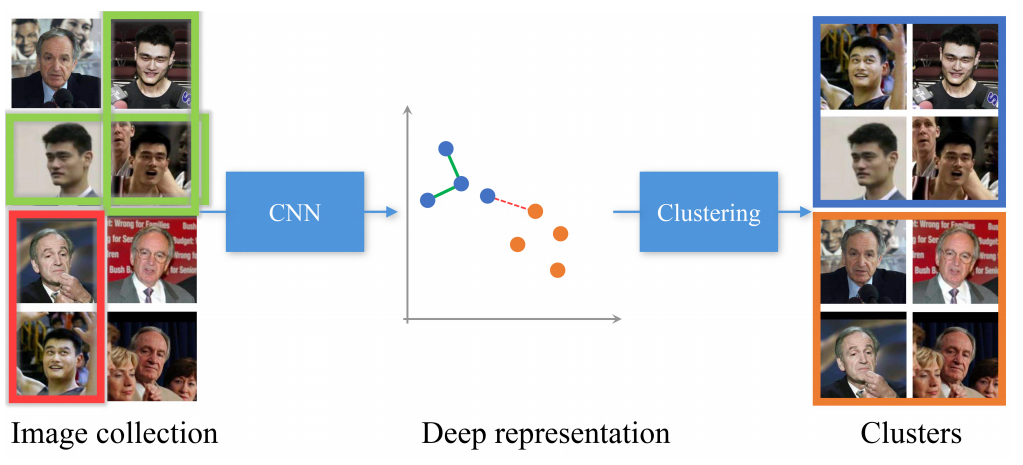
\includegraphics[width=\textwidth]{figures/otto_faceClustering_workflow.png}
    \caption{Face clustering workflow \cite{shi}}
	\label{fig:face}
\end{figure}

\section{Related Work}	

\subsection{Face Recognition}

\quad 
Face recognition focuses on identifying or verifying the identity of subjects in images or videos \cite{trigueros}.\\

Face recognition systems are usually composed of the following 4 steps \cite{trigueros}: 

\begin{enumerate}
  \item \textbf{Face Detection:}\\ Detect the position of the faces in an image and returns the coordinates of a bounding box for each face as shown in Figure \ref{fig:detect}.
  \item \textbf{Face Alignment:} \\ Find a set of facial landmarks with the best affine transformation that fits a set of reference points located at fixed locations in the image. As shown in Figure \ref{fig:landmark}, this step also includes resizing and cropping the image to the edges of the landmarks \cite{amos}. More specifically, as shown in Figure \ref{fig:meanlandmark} given a set of mean landmark locations, the affine transformation makes the landmarks detected in the face image close to the mean \cite{amos}.
  
  \item \textbf{Face Representation:} \\ Transform the pixel values of a face image into a low-dimensional discriminative feature vector, also known as an embedding. 
  \item \textbf{Face Matching:} \\ Compute similarity scores from feature vectors.
\end{enumerate} 
 
\begin{figure}[!tbp]
  \centering
  \begin{minipage}[b]{0.49\textwidth}
    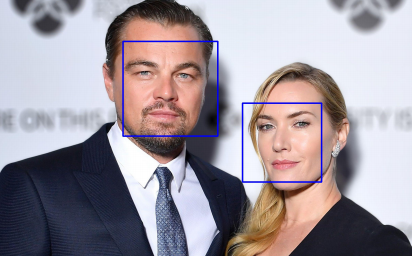
\includegraphics[width=\textwidth]{figures/face_detection.png}
    \caption{Face Detection \cite{trigueros}}
    \label{fig:detect}
  \end{minipage}
  \hfill
  \begin{minipage}[b]{0.49\textwidth}
    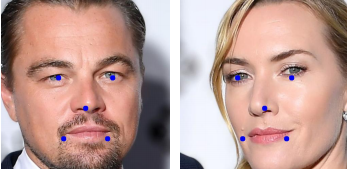
\includegraphics[width=\textwidth]{figures/landmark.png}
    \caption{Face Alignment \cite{trigueros}}
    \label{fig:landmark}
  \end{minipage}
\end{figure}

\begin{figure}[!tbp]
 \centering
    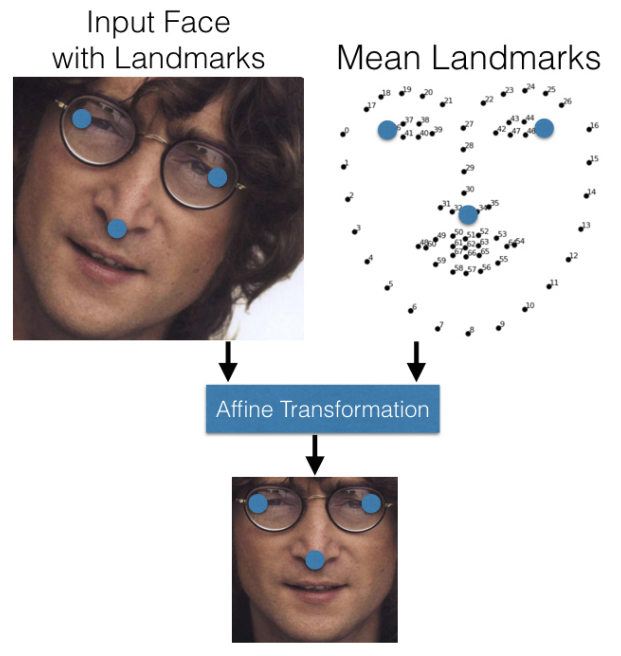
\includegraphics[width=0.7\textwidth]{figures/openface_detection.png}
    \caption{Applying affine transformation so that the face image is closer tothe set of mean landmarks. \cite{amos}}
	\label{fig:meanlandmark}
\end{figure}

\subsection{Face Detection}

\subsubsection{Histograms of Oriented Gradients}

\quad

A traditional method for face detection is the Histograms of Oriented Gradients (HOG) descriptors, which utilizes the distribution of local intensity gradients or edge directions to characterize local object appearance and shape in an image. HOG divides the image into small grids, where each grid accumulates a histogram of gradient directions or edge orientations over the pixels of the cell. The combination of all the histogram in the cells form the face region. The cells are then normalized for better invariance to illumination, shadowing, and other variations. The normalized local histograms of image gradient orientations in a dense grid as features are then trained to classify the region of the face in an image \cite{dalal}. When encountering a HOG representation of a new face image as shown in Figure \ref{fig:obama}, the part of the image that looks most similar to a trained HOG detector as shown in Figure \ref{fig:dlibhog} will form the region of the face. 

\begin{figure}[!tbp]
  \centering
  \begin{minipage}[b]{0.35\textwidth}
    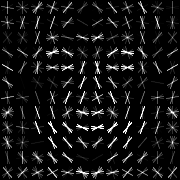
\includegraphics[width=\textwidth]{figures/hog_dlib.png}
    \caption{Trained HOG detector on multiple faces \cite{trigueros}}
    \label{fig:dlibhog}
  \end{minipage}
  \hfill
  \begin{minipage}[b]{0.45\textwidth}
    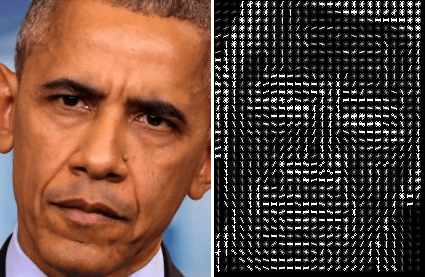
\includegraphics[width=\textwidth]{figures/face_hog.png}
    \caption{Hog representation of a face \cite{hackevolve}}
    \label{fig:obama}
  \end{minipage}
\end{figure}

\subsubsection{Multi-task Cascaded Convolutional Networks}

Another than using the tradition HOG representation and landmark detectors, face detection and alignment can also be done using CNNs. In particular, Multi-task Cascaded Convolutional Networks (MTCNN) is a widely used method to predict face and landmark location. The framework has a cascaded structure with three stages of deep CNNs shown in Figure \ref{fig:mtcnn}. \cite{zhang} 

The image is first resized to different scales to build an image pyramid and is the input of the three stages:

\begin{enumerate}
\item \textbf{Proposal Network (P-Net):} Obtain candidates that will serve as potential positions of the bounding boxes \cite{chinapas}.
%Obtains candidate windows and their bounding box regression vectors. The estimated bounding box regression vectors are used to calibrate the candidates. Then the bounding boxes are post-processed and filtered by the non-maximum suppression (NMS) algorithm to merge overlapped candidates.

\item \textbf{Refine Network (R-Net):} Using the image and the results of the first prediction of the bounding boxes, reduce false positives to get the final box boundaries \cite{chinapas}.
%Rejects false candidates, calibrates the candidates with bounding box regression, and NMS candidate merge.

\item \textbf{Output Network (O-Net):} Outputs five facial landmark positions \cite{zhang}.

\end{enumerate}

Both the predicting the bounding box regression and facial landmark localization uses regression to minimize the Euclidean loss between the candidate positions of the bounding boxes, landmark coordinates and the ground truth. The ground truth of the bounding boxes are the left, top, height, width of the box. The ground truth of the facial landmarks are the coordinates of the left, right eye, nose, left and right mouth corner \cite{zhang}.


\begin{figure}[!tbp]
 \centering
    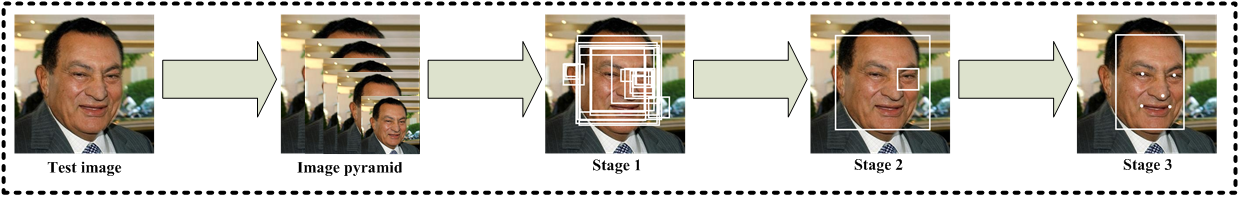
\includegraphics[width=\columnwidth]{figures/mtcnn_pipeline2.png}
    \caption{MTCNN: Cascaded structure with three stages of deep CNNs. \cite{zhang}}
	\label{fig:mtcnn}
\end{figure}


\subsection{Face Representation}

\quad
Face representation is conceivably the most important component in the system. However, challenges occur in real world (in-the-wild) images due to variations ranging from head poses and illumination conditions to aging and facial expressions \cite{trigueros}.

Traditional techniques include using statistical methods such as Principal Component Analysis (PCA) to represent faces as a combination of eigenvectors \cite{amos}. The top-performing face representation techniques use deep learning methods based on convolutional neural networks (CNNs) \cite{amos} since they are able to achieve very high accuracy by learning robust features due to the availability of large-scale faces in-the-wild datasets on the web \cite{trigueros}.  

\subsubsection{Convolutional Neural Networks}
\quad
As shown in Figure \ref{fig:nnflow} a neural network feeds the input into many layers of function compositions followed by a loss function which measures how well the neural network models the data. Each layer is parameterized by a vector or matrix $\theta_{i}$ and the aim is to optimize the loss function iteratively by finding the optimal gradients $\delta L \mathbin{/} \delta  \theta_{i}$ which are computed with the backpropagation \cite{amos}. 

Residual networks (ResNets) is a popular network architecture for face recognition. ResNets introduces a shortcut connection to learn a residual mapping which contributes to information flow across layers and allows the training of much deeper architectures \cite{trigueros}.

A common approach to training CNN models for face recognition is use a classification approach, where each face image in the training set corresponds to a class. When recognizing a new face image, the classification layer is discarded and the features of the previous layer are used as face representations. The downsides of this approach is that it doesn't generalize well to new face faces and that the representation size per face is large and inefficient \cite{schroff}.

Another approach is to learn the features for face representation directly by optimizing the distance between pairs or triplets of faces, in which the distances measure the similarity between faces \cite{trigueros} \cite{schroff}. 

\begin{figure}[!tbp]
 \centering
    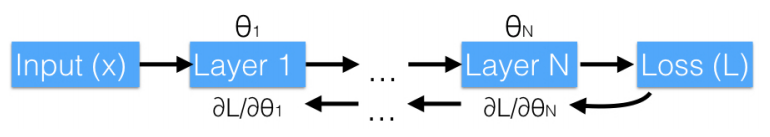
\includegraphics[width=\columnwidth]{figures/neural_flow.png}
    \caption{Neural Network Traing Flow. \cite{amos}}
	\label{fig:nnflow}
\end{figure}

\subsubsection{Triplet Loss Function}

\quad
When learning the face features directly, the choice of loss function has a great influence on the accuracy. One of the most used metric is the triplet loss function. The goal of the loss is to separate the distance between two aligned matching (positive) face images and a non-matching aligned (negative) face image by a distance margin. The result is a feature vector $f(x)$, known as embeddings, from a face image $x$ to a compact Euclidean feature space in $ \mathbb{R}^{d}$. The distance of the embeddings will be small if the faces are identical and large if the faces are distinct \cite{schroff}.


More specifically, as shown in the example in Figure \ref{fig:bale}. the distance between an anchor face image, $x_{i}^{a}$ is minimized by the loss and will be closer to all other positive face images $x_{i}^{p}$ than the negative face images $x_{i}^{n}$ where the distance is maximized by the loss. For each triplet $i$, the following condition needs to be satisfied: $$\Vert f(x_{i}^{a}) - f(x_{i}^{p}) \Vert_{2}^{2} + \alpha < \Vert f(x_{i}^{a}) - f(x_{i}^{n}) \Vert_{2}^{2} $$
where $\alpha$ is a margin that from the positive and negative pairs \cite{trigueros}.

For $N$ possible triplets, the loss being minimized is: $$ L = \sum_{i}^{N} \Big[ \Vert f(x_{i}^{a}) - f(x_{i}^{p}) \Vert_{2}^{2} - \Vert f(x_{i}^{a}) - f(x_{i}^{n}) \Vert_{2}^{2} + \alpha\Big]_{+} $$ \cite{schroff}.

As shown in Figure \ref{fig:loss} using a neural network, the triplet loss is computed and it's gradient is backpropagated through the network to the unique images \cite{amos}.

\begin{figure}[!tbp]
 \centering
    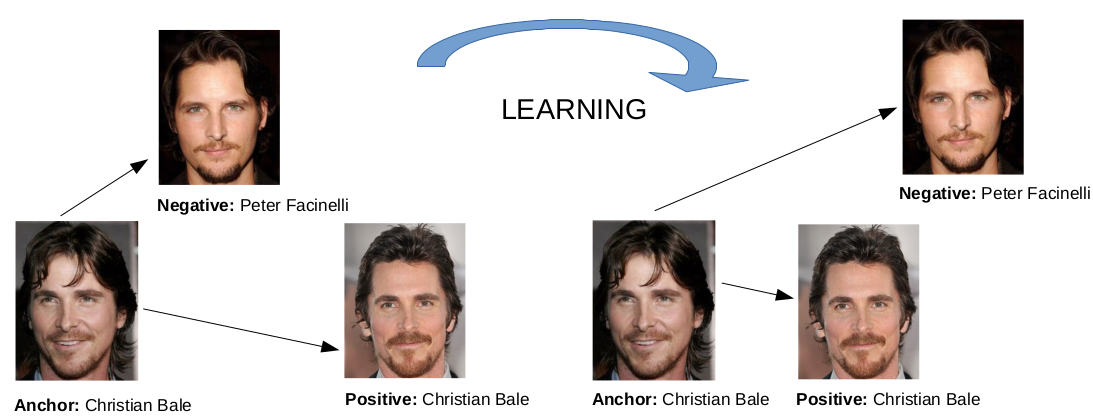
\includegraphics[width=0.8\textwidth]{figures/triplet_loss_example.png}
    \caption{The loss of identical faces are minimized and the loss of distinct faces are maximized by the triplet loss function \cite{pic1} \cite{pic2}.}
	\label{fig:bale}
\end{figure}

\begin{figure}[!tbp]
 \centering
    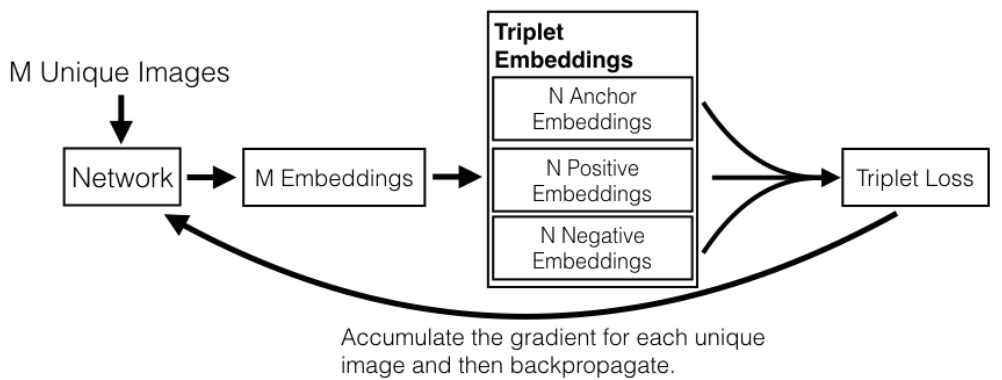
\includegraphics[width=0.7\columnwidth]{figures/openface_architecture.png}
    \caption{Learning the embeddings by optimizing the gradients of the triplet loss function \cite{amos}.}
	\label{fig:loss}
\end{figure}
 
\section{Face Representation Methods}
\label{facemethod}

The following section examines open-source state-of-the-art face feature extraction methods.

\subsection{FaceNet}

\quad

FaceNet is a method that uses a deep CNN along with the GoogLeNet style Inception models and the triplet loss function to directly optimize the face embeddings. The faces of images are first detected and aligned with MTCNN \cite{sandberg}, the resulting face images are 160 x 160 pixels and serve as the input for the FaceNet model. The structure of FaceNet consists of a batch input layer and a deep CNN followed by $L_{2}$ normalization, which results in the face embedding. This is followed by the triplet loss during training as shown in Figure \ref{fig:facemodel} \cite{schroff}.

Between 100 to 200 million face images consisting of about 8 million different identities were used for training. The large dataset of labelled faces consist of various poses, illuminations, and other variations. \cite{schroff}.

The pre-trained model (20180402-114759) of open-source FaceNet implementation \cite{sandberg} used in the experiment from Section \ref{experiment} was trained using the VGGFace2 dataset. The faces of the dataset was detected and aligned using MTCNN . The dataset contains 3.31 million images of 9131 identities, with an average of 362.6 images for each person. The images were downloaded from Google Image Search and have large variations in pose, age, illumination, ethnicity and profession. The model uses the Inception ResNet v1 architecture and has an accuracy of $99.65\%$ on the Labeled Faces in the Wild (LFW) benchmark \cite{sandberg}. \cite{sandberg}'s implementation results in a 512-dimensional feature vector.

\subsection{Dlib}
\quad
\cite{geitgey} built a face recognition method using Dlib-ml, which is an open source library for developing machine learning software in C++ \cite{king}. \cite{geitgey} used the HOG face detector from Dlib, which the HOG representation was trained with a linear classifier (SVM) \cite{king2014}. The face representation model uses the ResNet architecture with 29 convolution layers and the triplet loss function to learn the embeddings \cite{king2017}. The resulting feature embedding is a 128-dimensional vector \cite{king2017}. 

A dataset of about 3 million faces and 7485 unique identities from a combination of the face scrub and VGG dataset as well as a large number of other images scraped from the internet was used for training. The pre-trained model has an accuracy of $99.38\%$ on the LFW benchmark \cite{king2017}.

\begin{figure}[!tbp]
 \centering
    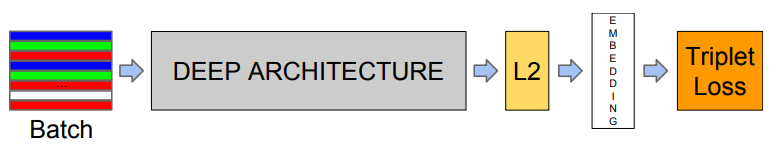
\includegraphics[width=\textwidth]{figures/facenet_model_archi.png}
    \caption{FaceNet model structure \cite{amos}}
	\label{fig:facemodel}
\end{figure}

\subsection{OpenFace}
\quad
OpenFace uses Dlib for face detection and alignment. The input images after alignment are 96 x 96 pixels. OpenFace was trained with 500,000 images from a combination of CASIA-WebFace and FaceScrub. The face representation is obtained using a modification of FaceNet's architecture, which the number of parameters are reduced. The resulting feature embedding is a 128 dimensional vector \cite{amos}.

\subsection{ArcFace}
\quad
\cite{deng} introduced a new loss function, additive angular margin (ArcFace), that uses a geometric interpretation for learning the discriminative features for face representation \cite{deng}. After applying MTCNN for face detection and alignment \cite{deng2019} get the 112 x 112 face input images, ArcFace further adjusts a face image by rotating an image to a straight face as shown in the comparsion in Figure \ref{fig:arcface1}. Consequently, the positions of eyebrows, eyes, nose, and mouth in different images are consistent and increases the effective when computing the similarities between the embeddings. The resulting embedding is a 512-dimensional vector \cite{deng}.

A downside of ArcFace is that it cannot compute face representations of images with the high intensity of light reflection \cite{chinapas} as shown in Figure \ref{fig:arcface2}.

The model is trained on MS1MV2 which is a refinement of the MS-Celeb-1M dataset. The training dataset contains about 10 million images of 100,000 top celebrities selected from one million celebrities in terms of their web appearance frequency \cite{deng}. The pre-trained model (LResNet100E-IR) used in the experiment in the next section was trained on the MS1MV2 dataset using the ResNet100 architecture which achieved an accuracy of $0.9982$ on the LFW benchmark \cite{deng2019}.

\begin{figure}[!tbp]
 \centering
    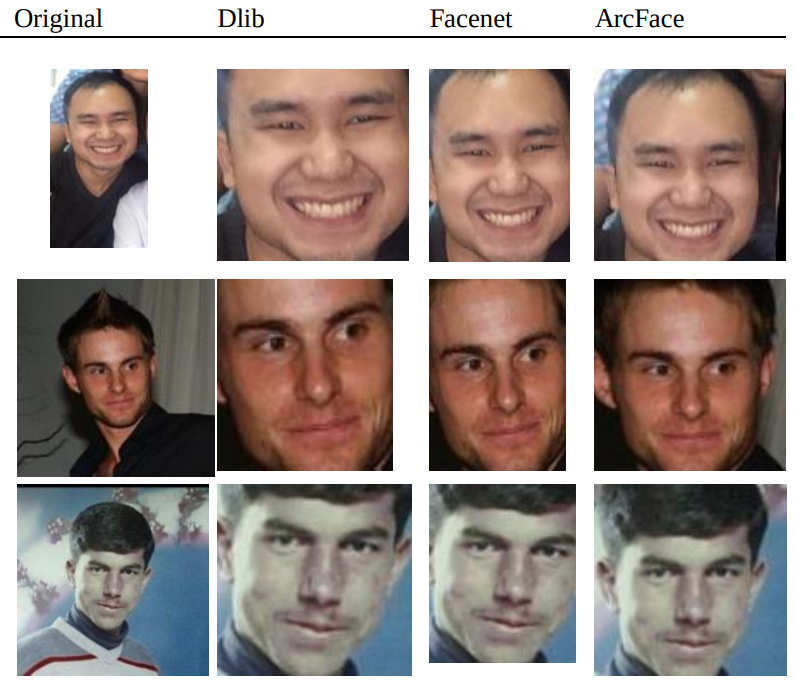
\includegraphics[width=0.6\textwidth]{figures/comparison.png}
    \caption{Comparsion of Face Detection between Dlib, FaceNet, and ArcFace \cite{chinapas}}
	\label{fig:arcface1}
\end{figure}

\begin{figure}[!tbp]
 \centering
    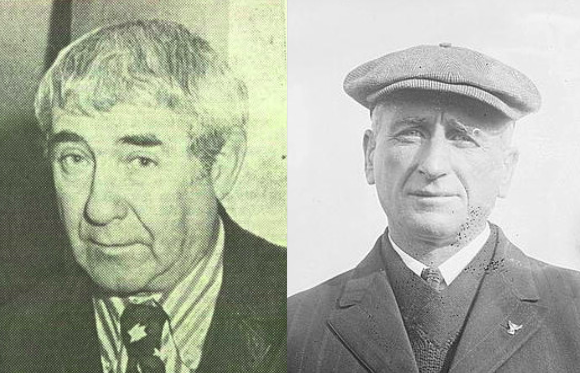
\includegraphics[width=0.6\textwidth]{figures/ex.png}
    \caption{Images with high intensity of light reflection in which ArcFace is unable to compute the embeddings for \cite{chinapas}}
	\label{fig:arcface2}
\end{figure}

\section{Clustering Algorithms}
\label{clustering}

\quad
Clustering can be considered the most important unsupervised learning problem and aims to find a structure in a collection of unlabeled data. Objects that are similar between each other are grouped in the same cluster, while dissimilar objects belong to other clusters \cite{ncbi}.


After obtaining the face embeddings, each face represents a data point in the dataset. The similarity between each face can therefore be computed and grouped using different metrics clustering algorithms. The following section will present the algorithms use in Section 5. 

\subsection{K-Means}

\quad
Lloyd’s K-Means algorithm is a commonly used clustering method due to it's simplicity and efficiency. It aims to minimize the average squared distance between points in the same cluster \cite{kmeans}. The algorithm first initializes k random centroids, which are random datapoints chosen from the dataset. Then each point is assigned to the closest centroid. The centroids are then recomputed as the average of all datapoints assigned to it. The latter two steps are repeated until the centroids don't change significantly. The implementation in \cite{scikit-learn} computes the difference between the old and new centroids and terminates until the difference is less than a threshold of $0.0001$ \cite{kmeans}.

Even though the converagence of this algorithm is guranteed, one of the drawbacks is that it assumes the datapoints of the clusters have the same variation, therefore responding poorly to clusters with irregular shapes. Moreover, the algorithm is highly sensitve to the initialization of the centroids which can noteably affect the accuracy of the clusters \cite{scikit-learn}. K-means++ is a method developed by \cite{kmeans} to address this issue, in which it initializes the centroids at random from the data points, but weights the data points from the closest centroid already chosen \cite{kmeans}. Therefore, the initialized centroids will be (generally) far from each other \cite{scikit-learn}. Experiments from \cite{kmeans} show that k-means++ outperforms k-means in terms of both accuracy and speed.

TODO: plots of bad initialization

\subsection{Spectral}

\quad
Spectral Clustering is an efficient clustering algorithm where it uses a low-dimensional embedding of the distance matrix between the data points, followed by the K-Means algorithm in the low dimensional space \cite{scikit-learn}.

\subsection{Hierarchical Agglomerative}

\quad
Hierarchical clustering is a method that merges or splits the clusters successively to form a nested tree of clusters, known as the dendrogram. In particular, Hierarchical Agglomerative Clustering is a bottom up approach where the root of the tree consists of the data points as their own clusters, then the clusters are successively merged together to form unique clusters at the leaves \cite{scikit-learn}.

The merging technique is determined by the linkage criteria. Section 5 uses Ward's method for the linkage criteria, in which it minimizes the variance of the clusters by the sum of squared differences. Although Ward's method gives the clusters the most regular sizes, the distance used in the clustering is limited to Euclidean metrics \cite{scikit-learn}.

\subsection{Expectation–Maximization}

The Expectation–Maximization (EM) algorithm is based on the Gaussian mixture model (GMM), which is a probabilistic method that assumes all the data points are generated from a mixture of Gaussian distributions with unknown latent parameters (mean, covariance) for each distribution \cite{scikit-learn}. The Gaussian distributions corresponds to the clusters and since the information of which distribution each data point belongs to is unknown the goal of the EM algorithm is to estimate the latent parameters for each distribution. After randomly initializing the latent parameters, EM executes the following two steps until convergence \cite{scikit-learn}.

\begin{enumerate}
\item \textbf{Expectation: } For each data point, compute the probability of it being generated by each latent parameter of the model. Each data point is then assigned to a cluster based on the probability.

\item \textbf{Maximize: } Re-estimate the latent parameters using the by maximizing the likelihood of the data given the assignments 

\end{enumerate}

The EM algorithm is similar to K-means, but instead the assignment of data points uses soft clustering. Instead of being either in a cluster or not (hard clustering), EM computes a probability of for assigning the data points \cite{ncbi}.

\subsection{Birch}

\quad
Birch clustering is an efficient data reduction algorithm in which it reduces the input data to a set of subclusters. For a given dataset, the algorithm builds the Characteristic Feature Tree (CFT) where the data points are compressed to a set of  Characteristic Feature nodes (CF Nodes). When a new data point is inserted into the CF Tree, it is merged with the nearest leaf of the subcluster of the root. These subclusters contain the necessary information for clustering \cite{scikit-learn}

\section{Experiment}
\label{experiment}

\subsection{Dataset}

\subsubsection{Experiment 1: Head shots of 5 types of athletes}
\label{experiment1}
\quad
This dataset consists of $2,180$ unique images of five categories of athletes obtained from a combination of repositories of \cite{data1}. As shown in Figure \ref{fig:sport}, \cite{data1} scraped the images directly from the official sport competition websites, therefore, the images are all high quality straight head shots \cite{data1}. The following shows the distribution of images:

\begin{itemize}
\item \textbf{NBA Basketball Players: } $225$ images
\item \textbf{UFC Fighting Champions: } $560$ images
\item \textbf{FIFA Soccer Players: } $735$ images
\item \textbf{PGA TOUR Golf Players: } $558$ images
\item \textbf{ATP Tour Tennis Players: } $102$ images
\end{itemize}


\begin{figure}[!tbp]
 \centering
    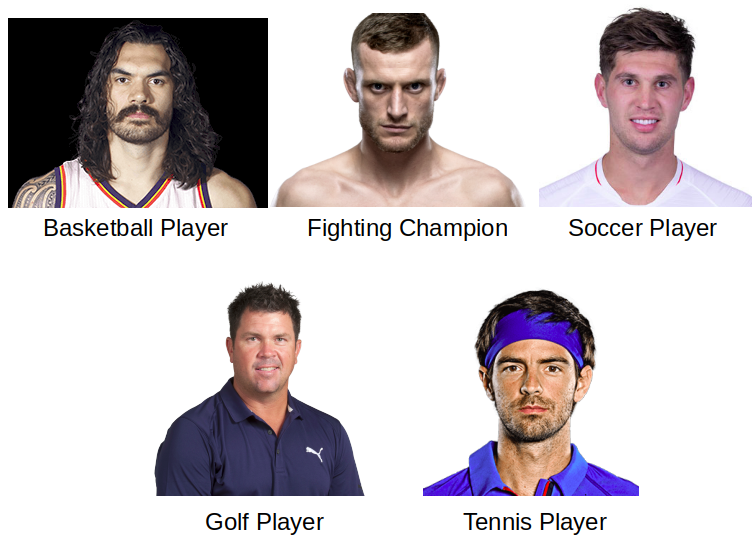
\includegraphics[width=0.7\columnwidth]{figures/ex1.png}
    \caption{Example of face images from the dataset of Experiment 1: Five categories of athletes \cite{data1}}
	\label{fig:sport}
\end{figure}

\subsubsection{Experiment 2: In-The-Wild images of 5 varying professions}
\label{experiment2}
\quad
This dataset consists of $2,065$ unique images of five different categories of professions. It is a combination of a subset of the dataset from \ref{experiment1} and a new dataset acquired using Wikidata's SPARQL query service. 

Wikidata is an open-source knowledge base for structured data. After choosing the professions and finding their entity ID's a query was formed to find people and the corresponding image links with of the occupation. In order to reduce variation in the dataset, additional queries were composed to obtain only males from North America and Europe. Since clustering algorithms like K-Means tend to generate similar sized clusters \cite{shi}, the number of images for each occupation are limited to similar sizes. An example of a query for the manager occupation can be found in \ref{appen1}. Then, the images were automatically downloaded using Python. As shown in Figure \ref{fig:prof}, opposed to the dataset from \ref{experiment1}, the images from Wikidata are in-the-wild images with varying head poses, illumination conditions, and other variations. The following shows the distribution of images:

\begin{itemize}
\item \textbf{Managers: } $371$ images
\item \textbf{Politicians: } $449$ images
\item \textbf{Military Officers: } $407$ images
\item \textbf{Architects: } $388$ images
\item \textbf{FIFA Soccer Players: } $450$ images
\end{itemize}

\begin{figure}[!tbp]
 \centering
    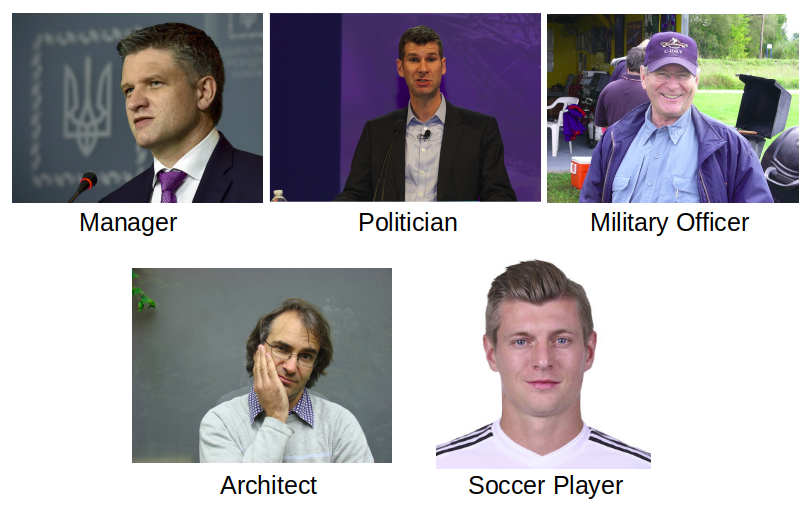
\includegraphics[width=0.7\columnwidth]{figures/ex2.png}
    \caption{Example of face images from the dataset of Experiment 2: Five categories of professions \cite{data1}}
	\label{fig:prof}
\end{figure}

\subsubsection{Experiment 3: In-The-Wild images of 11 varying professions}

\quad
This dataset consists of $4,593$ unique images of 11 different categories of professions. It is again a combination of a subset of the dataset from \ref{experiment1}, \ref{experiment2}, and images of five more professions downloaded from Wikidata using the same method as \ref{experiment2}. The following shows the distribution of images:

\begin{itemize}
\item \textbf{Managers: } $371$ images
\item \textbf{Entrepreneur: } $485$ images
\item \textbf{Politicians: } $449$ images
\item \textbf{Lawyer: } $394$ images
\item \textbf{Military Officers: } $407$ images
\item \textbf{Sport Coaches: } $334$ images
\item \textbf{FIFA Soccer Players: } $450$ images
\item \textbf{UFC Fighting Champions: } $537$ images
\item \textbf{Architects: } $388$ images
\item \textbf{Actor: } $403$ images
\item \textbf{Musician: } $375$ images

\begin{figure}[!tbp]
 \centering
    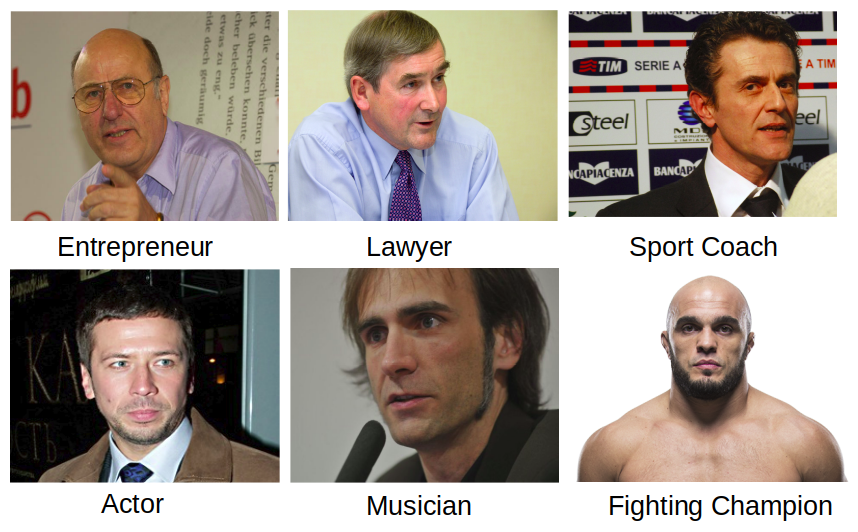
\includegraphics[width=0.7\columnwidth]{figures/ex3.png}
    \caption{Example of a subset of face images from the dataset of Experiment 3. In combination with \ref{fig:prof}, the professions make up the 11 professions for Experiment 3}
\end{figure}

\end{itemize}


\subsection{Set-Up}
\quad
In the experiments faces of people are clustered by profession using different clustering algorithms. Since the number of different professions are known, the number of clusters selected corresponds to the number of professions in each experiment. The cluster algorithms were applied to the feature embeddings using the methods described in Section \ref{facemethod}. Pre-trained models from each method was used in the experiment. 

\subsection{Framework}
\quad
Computer Device Details:
\begin{itemize}
\item Processor: Intel Core i5-4570 CPU, 3.20GHz x 4
\item 16 GB RAM
\end{itemize}

The following describes the steps to obtain the results:

\begin{enumerate}
\item \textbf{Load Images: } Each image is located inside a directory with the same filename
\item \textbf{Face Detection: } The FaceNet implementation uses MTCNN and the detected faces are of 160 x 160 pixels. Dlib uses the HOG face detector. OpenFace uses the HOG detector and the detected faces are of 96 x 96 pixels. ArcFace uses MTCNN and the detected faces are 112 x 112 pixels. Based on the open-source implementations, \cite{sandberg}, \cite{geitgey}, \cite{amos2016}, \cite{deng2019}, Table \ref{table:1} shows which face detection method was used for each method and the number of features in the resulting embeddings. Table \ref{table:2} shows the details of the accuracy based on the LWF benchmark, data size, and architecture of the pre-trained models.

\begin{table}[h!]
\centering
\begin{tabular}{||c c c||} 
 \hline
  Method & Face Detector & Number of Features\\ [0.5ex]
 \hline\hline
 \textbf{FaceNet} & MTCNN (160 x 160 px) & 512\\ 
 \hline
 \textbf{Dlib} & HOG & 128\\
 \hline
 \textbf{OpenFace} & HOG (96 x 96 px) & 128\\
 \hline
 \textbf{ArcFace} & MTCNN (112 x 112 px) & 512\\
 \hline
\end{tabular}
\caption{The face detection method used and the number of features of the embeddings extracted from each method \cite{sandberg}, \cite{geitgey}, \cite{amos2016}, \cite{deng2019}.}
\label{table:1}
\end{table}

\begin{table}[h!]
%\centering
\begin{adjustwidth}{-2.5cm}{}
\begin{tabular}{||c c c c ||} 
 \hline
  Method & LWF Accuracy & Dataset Size & Architecture\\ [0.5ex]
 \hline\hline
 \textbf{FaceNet} & 0.9965 & 3.31 million images, 9,121 identities & Inception ResNet v1\\ 
 \hline
 \textbf{Dlib} & 0.9938 & 3 million images, 7,485 identities & ResNet 29\\
 \hline
 \textbf{OpenFace} & 0.9292 & 500,000 images & Inception ResNet v1 (modified)\\
 \hline
 \textbf{ArcFace} & 0.9982 & 10 million images, 100,000 identities & ResNet 100\\
 \hline
 \textbf{Human-Level} \cite{amos} & 0.9753 &  &\\
 \hline
\end{tabular}
\caption{Accuracy based on the LWF benchmark, data size, and architecture of the pre-trained models \cite{sandberg}, \cite{geitgey}, \cite{amos2016}, \cite{deng2019}.}
\label{table:2}
\end{adjustwidth}
\end{table}


\item \textbf{Extract Feature Embeddings: } Using the pre-trained models provided by the implementations, the embeddings can be extracted. The embeddings of FaceNet and ArcFace both have 512 features and the embeddings of Dlib and OpenFace have 128 features. The embeddings and corresponding labels (identity and profession) of FaceNet, Dlib, and ArcFace are saved as binary files that can be loaded directly using NumPy in Python and the Openface embeddings and labels are saved as csv files. Table \ref{table:3} shows the dimensions of the feature embeddings extracted from each method.

\begin{table}[h!]
\centering
\begin{tabular}{||c c c c||} 
 \hline
  Method & Experiment 1 & Experiment 2 & Experiment 3\\ [0.5ex]
 \hline\hline
 \textbf{FaceNet} & 2,180 x 512 & 2,065 x 512 & 4,593 x 512\\ 
 \hline
 \textbf{Dlib} & 2,180 x 128 & 2,065 x 128 & 4,593 x 128\\
 \hline
 \textbf{OpenFace} & 2,180 x 128 & 2,065 x 128 & 4,593 x 128\\
 \hline
 \textbf{ArcFace} & 2,180 x 510 & 2,065 x 512 & 4,593 x 512\\
 \hline
\end{tabular}
\caption{Dimensions of the feature embeddings extracted from each method}
\label{table:3}
\end{table}

\item \textbf{Profession Clustering: } The clustering algorithms from Section \ref{clustering} were applied to the feature embeddings of the different methods. Since the number of different professions are known, the number of clusters selected corresponds to the number of professions in each experiment. The example in Figure \ref{fig:plot1} has two professions. After detecting the faces and representing them as embeddings, Figure \ref{fig:plot2} shows the clustering results. The embeddings are visualized using PCA.
\end{enumerate}

\begin{figure}[H]
  \centering
  \begin{minipage}[b]{0.3\textwidth}
    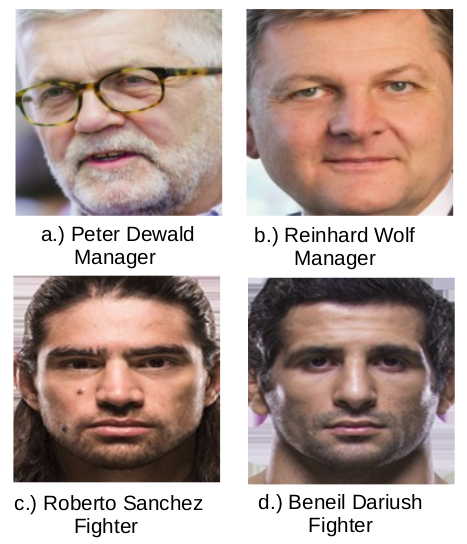
\includegraphics[width=\textwidth]{figures/plot2.png}
    \caption{The goal is to cluster the professions of the aligned images.}
    \label{fig:plot1}
  \end{minipage}
  \hfill
  \begin{minipage}[b]{0.6\textwidth}
    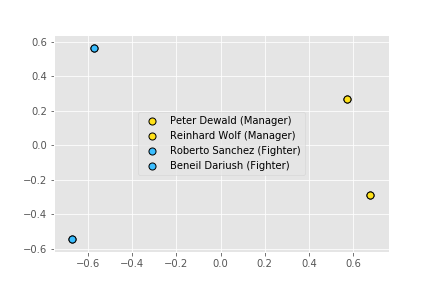
\includegraphics[width=\textwidth]{figures/plot.png}
    \caption{PCA plot after clustering using the embeddings of the faces from Figure \ref{fig:plot1}}
    \label{fig:plot2}
  \end{minipage}
\end{figure}

\begin{figure}[H]
 \centering
    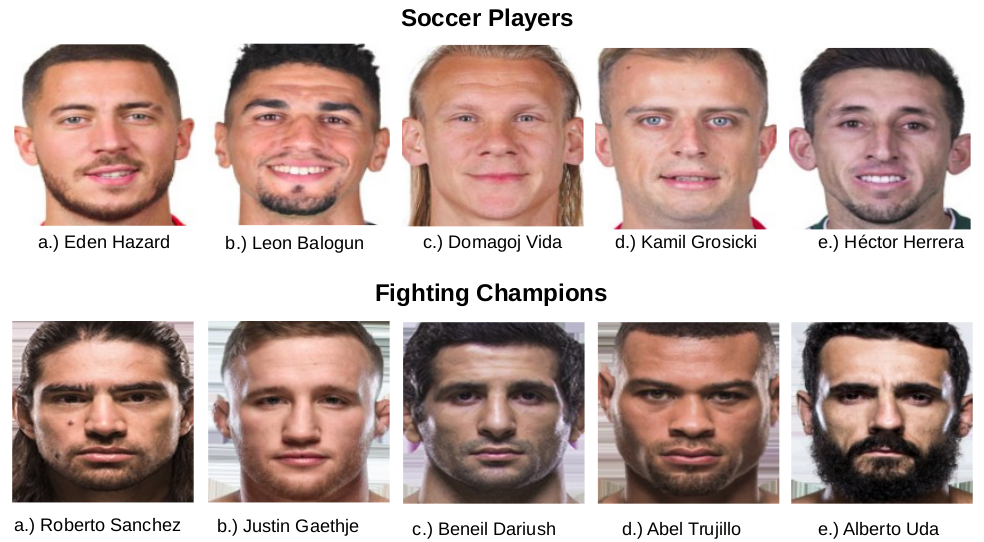
\includegraphics[width=\columnwidth]{figures/soccer_tp.png}
    \caption{\textbf{True Positives} using FaceNet and K-Means. Clusters of Soccer Players and Fighting Champions.}
    \label{fig:ex1tp}
\end{figure}


\section{Results}

\subsection{Evaluation}
\quad
Since the dataset provides the labels of the correct profession for each face image, the accuracy of the clusters can be evaluated corresponding to the known profession labels. Due to efficiency, the clustering accuracy is evaluated with the Pairwise F-Measure \cite{otto}.

\subsubsection{Pairwise F-Measure}

\begin{figure}[!tbp]
 \centering
    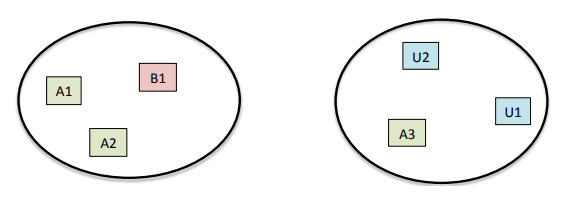
\includegraphics[width=\columnwidth]{figures/fmeasure.png}
    \caption{Example of a possible clustering output. Six data points are grouped into 2 clusters. A1, A2, and A3 have the same label, B1 has it's own label, and samples U1 and U2 have the same label \cite{otto}.}
    \label{fig:fmeasure}
\end{figure}

Suppose $L = \{l_{1},...,l_{n}\}$ contains the actual labels for each face and $C = \{c_{1},...,c_{n}\}$ are the labels from the output of the clustering algorithm. For example, shown in Figure \ref{fig:fmeasure}, the actual labels are $$L = \{\{A1, A2, A3\}, \{B1\}, \{U1, U2\}\}$$ and the labels from the output of the cluster algorithm are $$C = \{\{A1, A2, B1\}, \{A3, U1, U2 \}\}$$
Then the set of face pairs from the actual labels are $$P = \{(A1, A2), (A1, A3), (A2, A3), (U1, U2)\}$$ 
The set of face pairs from the labels of the cluster algorithm are $$Q = \{(A1, A2), (A1, B1), (A2, B1), (A3, U1), (A3, U2), (U1, U2)\}$$
For each face pair $(i, j)$ of each cluster \cite{thesis}: \\
\begin{itemize}
\item \textbf{True Positive (TP):} The number of face pairs $(i, j)$ that are correctly clustered into the same cluster.
$$TP = | \{(i, j) \ \textrm{where} \ c_{i} = c_{j} \ \textrm{and} \ l_{i} = l_{j}\}|$$

In Figure \ref{fig:fmeasure}, $(A1, A2), (U1, U2)$ are matching pairs and
$$TP = | P \cap Q | = |\{(A1, A2), (U1, U2)\}| = 2$$

\item \textbf{False Positives (FP):} The number of face pairs $(i, j)$ that are incorrectly clustered to the same cluster. $$FP = | \{(i, j) \ \textrm{where} \ c_{i} = c_{j} \ \textrm{and} \ l_{i} \neq l_{j}\}|$$

In Figure \ref{fig:fmeasure}, $(A1, B1), (A2, B1), (A3, U1), (A3, U2)$ are mismatching pairs and $$FP = |Q - P| = |\{(A1, B1), (A2, B1), (A3, U1), (A3, U2)\}| = 4$$ 

\item \textbf{False Negatives (FN)}: The number of face pairs that are clustered to a different cluster. $$TN = | \{(i, j) \ \textrm{where} \ c_{i} \neq c_{j} \ \textrm{and} \ l_{i} \neq l_{j}\}|$$

In Figure \ref{fig:fmeasure}, $(A1, A3), (A2, A3)$ are same-class pairs in different clusters and $$FN = |P - Q| = |\{(A1, A3), (A2, A3)\}| = 2$$
\end{itemize}


\begin{itemize}
\item \textbf{Pairwise Precision:} Fraction of face pairs that are correctly clustered together over the total number of pairs that belong to the same class \cite{shi}.
$$ Pairwise \ Precision = \frac{TP}{TP + FP}$$

\item \textbf{Pairwise Recall:} Fraction of face pairs that are correctly clustered together over the total number of pairs that are in the same cluster \cite{shi}.
$$ Pairwise \ Recall = \frac{TP}{TP + FN}$$

\item \textbf{Pairwise F-Measure:} Harmonic mean of Precision and Recall \cite{shi} $$Pairwise \ F\textrm{-}Measure = \frac{2 * \textrm{Precision}*\textrm{Recall}}{\textrm{Precision} + \textrm{Recall}}$$
\end{itemize}
If the output of the algorithm clusters all data points as individual clusters, it will have a high precision, but low recall. Whereas if the output clusters all data points in the same cluster, it will have a high recall, but low precision \cite{otto}.


%For example if $P = \{(1, 2), (1, 3), (2, 3), (4, 5)\}$ is a set of face pairs from the ground truth labels and $Q = \{(2, 3), (1, 4), (1, 5), (4, 5)\}$ is the set of face pairs from the labels of the clustering algorithms where the face pairs are represented by the indices of their embeddings. Then $$TP = | P \cap Q | = |\{(2, 3), (4, 5)\}| = 2$$ $$FP = |Q - P| = |\{(1, 4), (1, 5)\}| = 2$$ $$FN = |P - Q| = |\{(1, 2), (1, 3)\}| = 2$$

%\item \textbf{Create ground truth dictionary: } Based on the embeddings and labels from the feature extraction methods, a dictionary that assigns the indices of the images to the corresponding profession was created. The identity and profession can later be retrieved from the indices. The keys are the professions and the values are arrays of image indices. e.g. $\{\textrm{tennis player}: [41, 54, ...], \ \textrm{basketball player}: [0, 2, 5, ...], \ \textrm{golfer}: [...], ...\}$

\subsection{Experiment 1}

The results were obtained by averaging 10 F-measure scores. 

\begin{table}[h!]
\centering
\begin{tabular}{||c c c c c||} 
 \hline
Method & FaceNet & Dlib & OpenFace & ArcFace\\ [0.5ex]
 \hline\hline
 \textbf{K-Means} & 0.478 & 0.391 & 0.382 & \textbf{0.516}\\ 
 \hline
  \textbf{Spectral} & 0.445 & 0.361 & 0.345 & \textbf{0.467}\\
 \hline
 \textbf{HAC} & \textbf{0.447} & 0.362 & 0.391 & 0.413\\
 \hline
 \textbf{EM} & 0.449 & 0.394 & 0.376 & \textbf{0.512}\\
 \hline
 \textbf{Birch} & 0.442 & 0.404 & 0.331 & \textbf{0.453}\\
 \hline
\end{tabular}
\caption{Experiment 1: Comparison of Feature Extraction Methods and F-Measure of Clustering Algorithms}
\label{table:ex1}
\end{table}

\begin{itemize}
\item \textbf{FaceNet}
\begin{table}[H]
\centering
\begin{tabular}{||c c c c c c||} 
 \hline
 Clustering Method & \# of clusters & F-Measure & Precision & Recall & Runtime\\ [0.5ex]
 \hline\hline
 \textbf{K-Means} & 5 & \textbf{0.478} & 0.515 & 0.446 & 0.906\\ 
 \hline
  \textbf{Spectral} & 5 & 0.445 & 0.507 & 0.397 & 0.662\\
 \hline
 \textbf{HAC} & 5 & 0.447 & 0.463 & 0.432 & 0.669\\
 \hline
 \textbf{EM} & 5 & 0.449 & 0.499 & 0.408 & 5.004\\
 \hline
 \textbf{Birch} & 5 & 0.442 & 0.452 & 0.432 & 0.553\\
 \hline
\end{tabular}
\caption{Experiment 1 FaceNet}
\label{table:ex1facenet}
\end{table}

\item \textbf{Dlib}
\begin{table}[H]
\centering
\begin{tabular}{||c c c c c c||} 
 \hline
 Clustering Method & \# of clusters & F-Measure & Precision & Recall & Runtime\\ [0.5ex]
 \hline\hline
 \textbf{K-Means} & 5 & 0.391 & 0.415 & 0.370 & 0.277\\ 
 \hline
  \textbf{Spectral} & 5 & 0.361 & 0.385 & 0.339 & 0.631\\
 \hline
 \textbf{HAC} & 5 & 0.362 & 0.384 & 0.343 & 0.234\\
 \hline
 \textbf{EM} & 5 & 0.394 & 0.419 & 0.372 & 0.594\\
 \hline
 \textbf{Birch} & 5 & \textbf{0.404} & 0.325 & 0.533 & 0.086\\
 \hline
\end{tabular}
\caption{Experiment 1 Dlib}
\label{table:ex1dlib}
\end{table}

\item \textbf{OpenFace}
\begin{table}[H]
\centering
\begin{tabular}{||c c c c c c||} 
 \hline
 Clustering Method & \# of clusters & F-Measure & Precision & Recall & Runtime\\ [0.5ex]
 \hline\hline
 \textbf{K-Means} & 5 & 0.382 & 0.410 & 0.357 & 0.258\\ 
 \hline
  \textbf{Spectral} & 5 & 0.345 & 0.359 & 0.332 & 0.665\\
 \hline
 \textbf{HAC} & 5 & \textbf{0.391} & 0.369 & 0.417 & 0.226\\
 \hline
 \textbf{EM} & 5 & 0.376 & 0.408 & 0.349 & 0.475\\
 \hline
 \textbf{Birch} & 5 & 0.331 & 0.365 & 0.303 & 0.12\\
 \hline
\end{tabular}
\caption{Experiment 1 OpenFace}
\label{table:ex1openface}
\end{table}

\item \textbf{ArcFace}
\begin{table}[H]
\centering
\begin{tabular}{||c c c c c c||} 
 \hline
 Clustering Method & \# of clusters & F-Measure & Precision & Recall & Runtime\\ [0.5ex]
 \hline\hline
 \textbf{K-Means} & 5 & \textbf{0.516} & 0.588 & 0.459 & 1.211\\ 
 \hline
  \textbf{Spectral} & 5 & 0.467 & 0.533 & 0.415 & 0.804\\
 \hline
 \textbf{HAC} & 5 & 0.413 & 0.459 & 0.376 & 0.756\\
 \hline
 \textbf{EM} & 5 & 0.512 & 0.582 & 0.457 & 1.03\\
 \hline
 \textbf{Birch} & 5 & 0.453 & 0.473 & 0.434 & 1.036\\
 \hline
\end{tabular}
\caption{Experiment 1 ArFace}
\label{table:ex1arcface}
\end{table}

\end{itemize}


\begin{figure}[H]
 \centering
    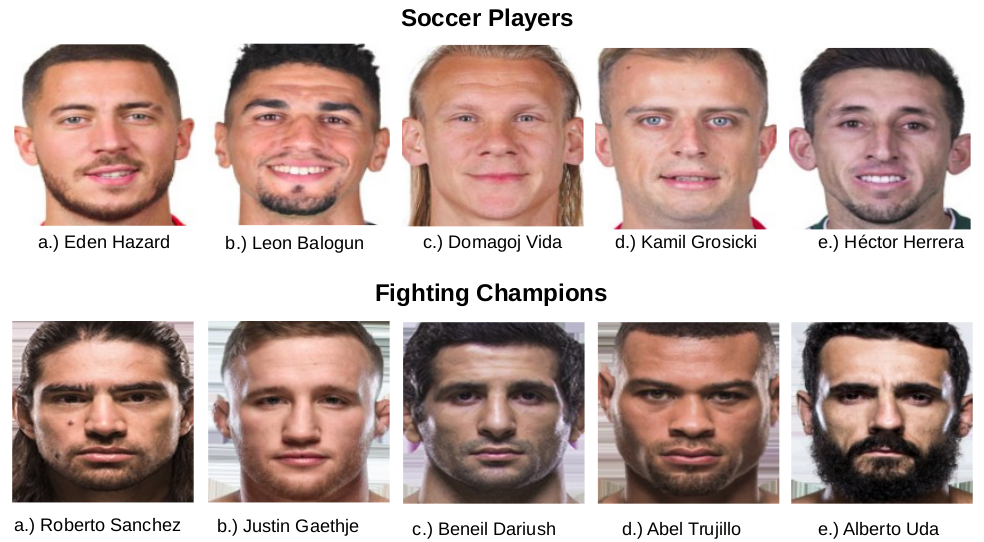
\includegraphics[width=\columnwidth]{figures/soccer_tp.png}
    \caption{\textbf{True Positives} using FaceNet and K-Means. Clusters of Soccer Players and Fighting Champions.}
    \label{fig:ex1tp}
\end{figure}

\begin{figure}[H]
  \centering
  \begin{minipage}[b]{0.4\textwidth}
    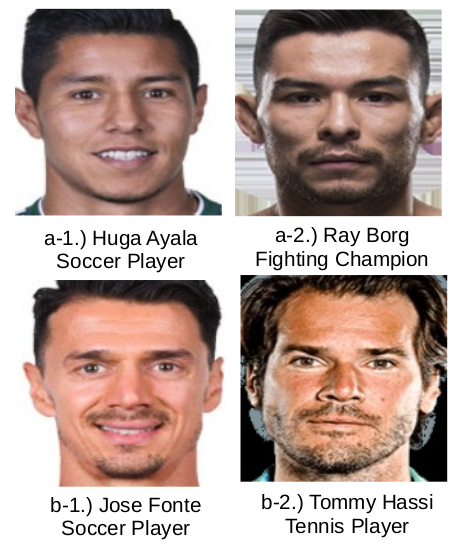
\includegraphics[width=\textwidth]{figures/soccer_fp.png}
    \caption{\textbf{False Positives}}
    \label{fig:ex1fp}
  \end{minipage}
  \hfill
  \begin{minipage}[b]{0.4\textwidth}
    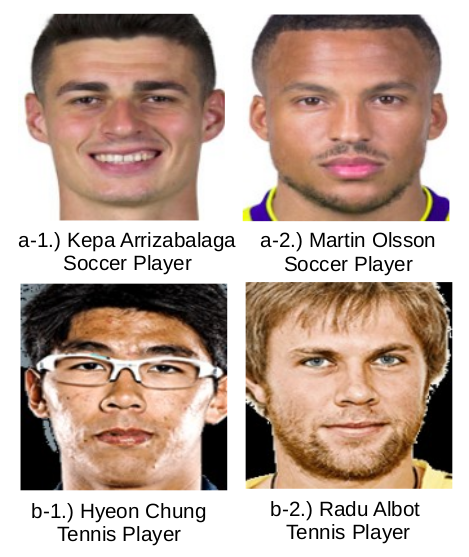
\includegraphics[width=\textwidth]{figures/soccer_fn.png}
    \caption{\textbf{False Negatives}}
    \label{fig:ex1fn}
  \end{minipage}
\end{figure}

\subsection{Experiment 2}

\begin{table}[H]
\centering
\begin{tabular}{||c c c c c||} 
 \hline
Method & FaceNet & Dlib & OpenFace & ArcFace\\ [0.5ex]
 \hline\hline
 \textbf{K-Means} & \textbf{0.426} & 0.405 & 0.306 & 0.294\\ 
 \hline
  \textbf{Spectral} & \textbf{0.392} & 0.367 & 0.295 & 0.272\\
 \hline
 \textbf{HAC} & 0.384 & \textbf{0.392} & 0.310 & 0.333\\
 \hline
 \textbf{EM} & \textbf{0.443} & 0.411 & 0.310 & 0.277\\
 \hline
 \textbf{Birch} & \textbf{0.399} & 0.383 & 0.294 & 0.304\\
 \hline
\end{tabular}
\caption{Experiment 2: Comparison of Feature Extraction Methods and F-Measure of Clustering Algorithms}
\label{table:ex2}
\end{table}

\begin{itemize}

\item \textbf{FaceNet}
\begin{table}[H]
\centering
\begin{tabular}{||c c c c c c||} 
 \hline
 Clustering Method & \# of clusters & F-Measure & Precision & Recall & Runtime\\ [0.5ex]
 \hline\hline
 \textbf{K-Means} & 5 & 0.426 & 0.415 & 0.439 & 0.880\\ 
 \hline
  \textbf{Spectral} & 5 & 0.392 & 0.379 & 0.408 & 0.617\\
 \hline
 \textbf{HAC} & 5 & 0.384 & 0.331 & 0.457 & 0.590\\
 \hline
 \textbf{EM} & 5 & \textbf{0.443} & 0.427 & 0.461 & 5.337\\
 \hline
 \textbf{Birch} & 5 & 0.399 & 0.368 & 0.435 & 0.499\\
 \hline
\end{tabular}
\caption{Experiment 2 FaceNet}
\label{table:ex2facenet}
\end{table}

\item \textbf{Dlib}
\begin{table}[H]
\centering
\begin{tabular}{||c c c c c c||} 
 \hline
 Clustering Method & \# of clusters & F-Measure & Precision & Recall & Runtime\\ [0.5ex]
 \hline\hline
 \textbf{K-Means} & 5 & \textbf{0.405} & 0.404 & 0.408 & 0.287\\ 
 \hline
  \textbf{Spectral} & 5 & 0.367 & 0.365 & 0.370 & 0.640\\
 \hline
 \textbf{HAC} & 5 & 0.392 & 0.348 & 0.450 & 0.201\\
 \hline
 \textbf{EM} & 5 & 0.411 & 0.401 & 0.422 & 0.532\\
 \hline
 \textbf{Birch} & 5 & 0.383 & 0.280 & 0.606 & 0.077\\
 \hline
\end{tabular}
\caption{Experiment 2 Dlib}
\label{table:ex2dlib}
\end{table}

\item \textbf{OpenFace}
\begin{table}[H]
\centering
\begin{tabular}{||c c c c c c||} 
 \hline
 Clustering Method & \# of clusters & F-Measure & Precision & Recall & Runtime\\ [0.5ex]
 \hline\hline
 \textbf{K-Means} & 5 & 0.306 & 0.306 & 0.307 & 0.344\\ 
 \hline
  \textbf{Spectral} & 5 & 0.295 & 0.293 & 0.297 & 0.624\\
 \hline
 \textbf{HAC} & 5 & \textbf{0.310} & 0.282 & 0.345 & 0.203\\
 \hline
 \textbf{EM} & 5 & \textbf{0.310} & 0.310 & 0.311 & 0.398\\
 \hline
 \textbf{Birch} & 5 & 0.294 & 0.276 & 0.314 & 0.137\\
 \hline
\end{tabular}
\caption{Experiment 2 OpenFace}
\label{table:ex2openface}
\end{table}

\item \textbf{ArcFace}
\begin{table}[H]
\centering
\begin{tabular}{||c c c c c c||} 
 \hline
 Clustering Method & \# of clusters & F-Measure & Precision & Recall & Runtime\\ [0.5ex]
 \hline\hline
 \textbf{K-Means} & 5 & 0.294 & 0.283 & 0.306 & 1.332\\ 
 \hline
  \textbf{Spectral} & 5 & 0.272 & 0.262 & 0.283 & 0.742\\
 \hline
 \textbf{HAC} & 5 & \textbf{0.333} & 0.277 & 0.418 & 0.586\\
 \hline
 \textbf{EM} & 5 & 0.277 & 0.268 & 0.288 & 0.803\\
 \hline
 \textbf{Birch} & 5 & 0.304 & 0.255 & 0.376 & 0.837\\
 \hline
\end{tabular}
\caption{Experiment 2 ArFace}
\label{table:ex2arcface}
\end{table}
\end{itemize}

\begin{figure}[!tbp]
 \centering
    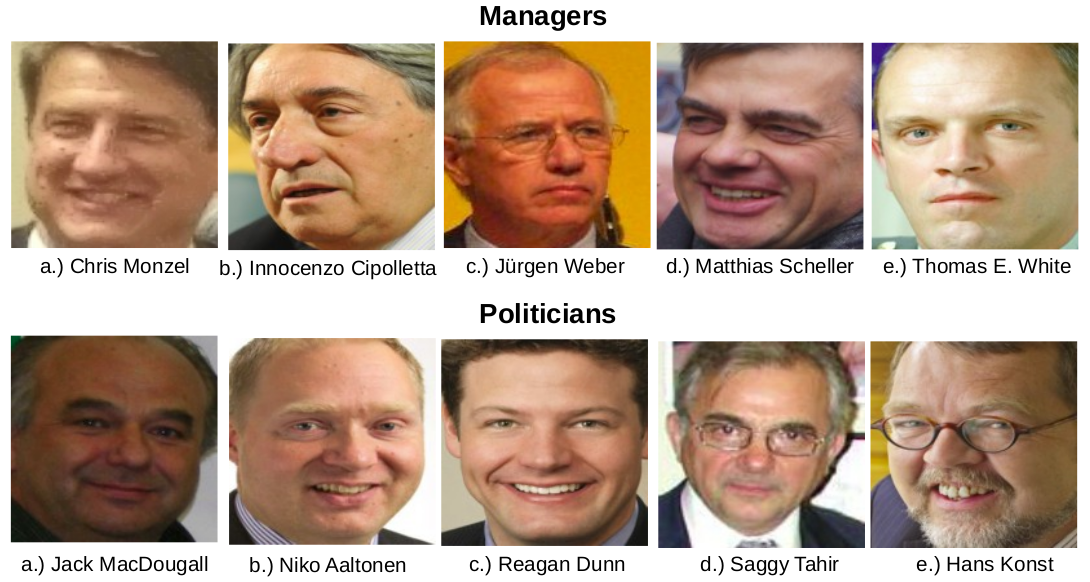
\includegraphics[width=\columnwidth]{figures/manager.png}
    \caption{Experiment 2: Cluster of Managers and Politicians}
    \label{fig:ex2tp}
\end{figure}

\begin{figure}[!tbp]
 \centering
    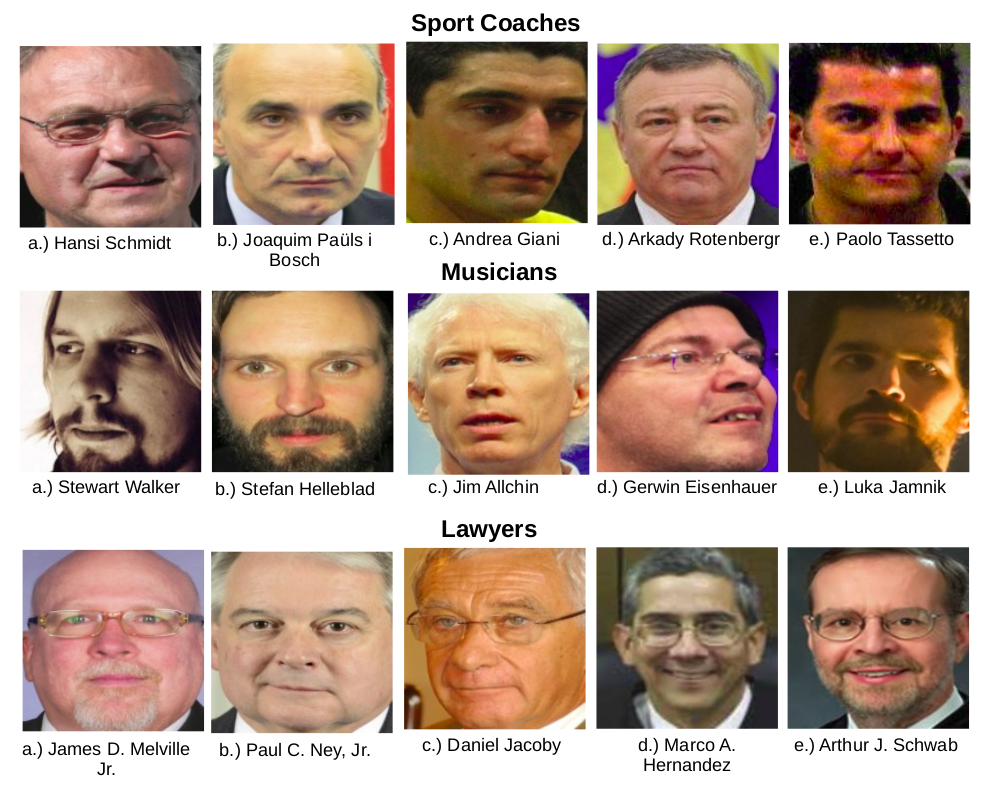
\includegraphics[width=\columnwidth]{figures/lawyers.png}
    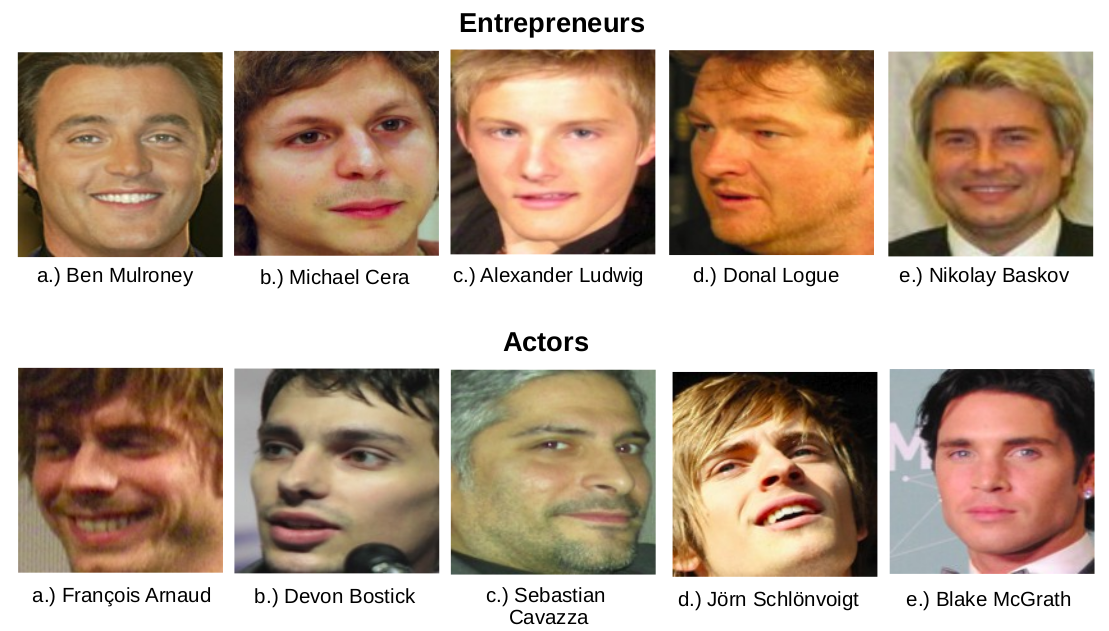
\includegraphics[width=\columnwidth]{figures/actor.png}
    \caption{Experiment 3: Cluster of Sport Coaches, Musicians, Lawyers, Entrepreneurs, and Actors}
    \label{fig:ex2tp}
\end{figure}

\begin{figure}[H]
  \centering
  \begin{minipage}[b]{0.48\textwidth}
    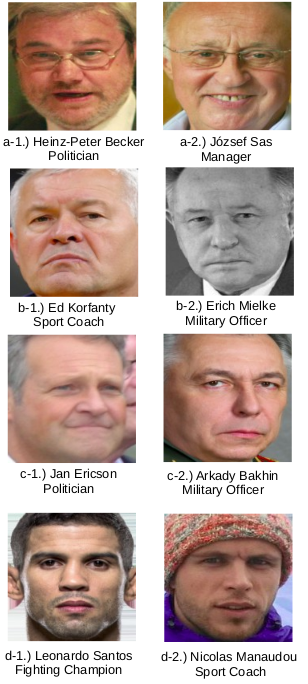
\includegraphics[width=\textwidth]{figures/ex2_fp.png}
    \caption{\textbf{False Positives}}
    \label{fig:ex2fp}
  \end{minipage}
  \hfill
  \begin{minipage}[b]{0.5\textwidth}
   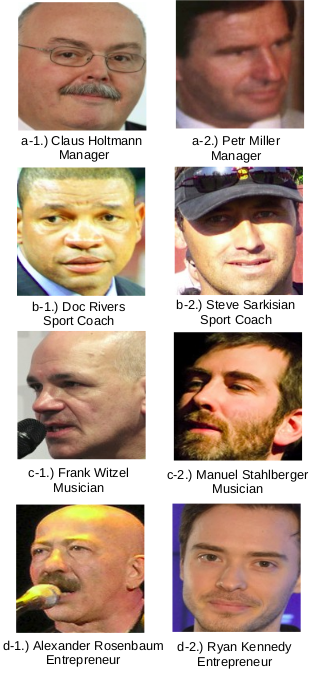
\includegraphics[width=\textwidth]{figures/ex2_fn.png}
    \caption{\textbf{False Negatives}}
    \label{fig:ex2fn}
  \end{minipage}
\end{figure}

\subsection{Experiment 3}

\begin{table}[H]
\centering
\begin{tabular}{||c c c c c||} 
 \hline
Method & FaceNet & Dlib & OpenFace & ArcFace\\ [0.5ex]
 \hline\hline
 \textbf{K-Means} & \textbf{0.203} & 0.185 & 0.141 & 0.182\\ 
 \hline
  \textbf{Spectral} & \textbf{0.204} & 0.166 & 0.143 & 0.159\\
 \hline
 \textbf{HAC} & 0.177 & \textbf{0.188} & 0.131 & 0.174\\
 \hline
 \textbf{EM} & \textbf{0.210} & 0.191 & 0.146 & 0.179\\
 \hline
 \textbf{Birch} & 0.182 & \textbf{0.193} & 0.149 & 0.151\\
 \hline
\end{tabular}
\caption{Experiment 3: Comparison of Feature Extraction Methods and F-Measure of Clustering Algorithms}
\label{table:ex3}
\end{table}

\begin{itemize}

\item \textbf{FaceNet}
\begin{table}[H]
\centering
\begin{tabular}{||c c c c c c||} 
 \hline
 Clustering Method & \# of clusters & F-Measure & Precision & Recall & Runtime (seconds)\\ [0.5ex]
 \hline\hline
 \textbf{K-Means} & 11 & 0.203 & 0.202 & 0.204 & 3.698\\ 
 \hline
  \textbf{Spectral} & 11 & 0.204 & 0.205 & 0.203 & 3.695\\
 \hline
 \textbf{HAC} & 11 & 0.177 & 0.154 & 0.209 & 3.497\\
 \hline
 \textbf{EM} & 11 & \textbf{0.210} & 0.206 & 0.215 & 25.618\\
 \hline
 \textbf{Birch} & 11 & 0.182 & 0.172 & 0.193 & 2.271\\
 \hline
\end{tabular}
\caption{Experiment 3 FaceNet}
\label{table:ex3facenet}
\end{table}

\item \textbf{Dlib}
\begin{table}[H]
\centering
\begin{tabular}{||c c c c c c||} 
 \hline
 Clustering Method & \# of clusters & F-Measure & Precision & Recall & Runtime (seconds)\\ [0.5ex]
 \hline\hline
 \textbf{K-Means} & 11 & 0.185 & 0.181 & 0.190 & 1.260\\ 
 \hline
  \textbf{Spectral} & 11 & 0.166 & 0.167 & 0.167 & 3.458\\
 \hline
 \textbf{HAC} & 11 & 0.188 & 0.168 & 0.214 & 1.132\\
 \hline
 \textbf{EM} & 11 & 0.191 & 0.186 & 0.196 & 3.296\\
 \hline
 \textbf{Birch} & 11 & \textbf{0.193} & 0.140 & 0.310 & 0.207\\
 \hline
\end{tabular}
\caption{Experiment 3 Dlib}
\label{table:ex3dlib}
\end{table}

\item \textbf{OpenFace}
\begin{table}[H]
\centering
\begin{tabular}{||c c c c c c||} 
 \hline
 Clustering Method & \# of clusters & F-Measure & Precision & Recall & Runtime (seconds)\\ [0.5ex]
 \hline\hline
 \textbf{K-Means} & 11 & 0.141 & 0.139 & 0.145 & 1.162\\ 
 \hline
  \textbf{Spectral} & 11 & 0.143 & 0.130 & 0.160 & 1.140\\
 \hline
 \textbf{HAC} & 11 & 0.131 & 0.130 & 0.133 & 3.500\\
 \hline
 \textbf{EM} & 11 & 0.146 & 0.143 & 0.150 & 3.233\\
 \hline
 \textbf{Birch} & 11 & \textbf{0.149} & 0.137 & 0.164 & 0.492\\
 \hline
\end{tabular}
\caption{Experiment 3 OpenFace}
\label{table:ex3openface}
\end{table}

\item \textbf{ArcFace}
\begin{table}[H]
\centering
\begin{tabular}{||c c c c c c||} 
 \hline
 Clustering Method & \# of clusters & F-Measure & Precision & Recall & Runtime (seconds)\\ [0.5ex]
 \hline\hline
 \textbf{K-Means} & 11 & \textbf{0.182} & 0.182 & 0.183 & 4.679\\ 
 \hline
  \textbf{Spectral} & 11 & 0.159 & 0.159 & 0.159 & 4.112\\
 \hline
 \textbf{HAC} & 11 & 0.174 & 0.156 & 0.197 & 3.600\\
 \hline
 \textbf{EM} & 11 & 0.179 & 0.178 & 0.180 & 4.043\\
 \hline
 \textbf{Birch} & 11 & 0.151 & 0.122 & 0.197 & 3.986\\
 \hline
\end{tabular}
\caption{Experiment 3 ArcFace}
\label{table:ex3arcface}
\end{table}

\end{itemize}

\subsection{Analysis}

\begin{table}[h!]
\centering
\begin{tabular}{||c c c c||} 
 \hline
Feature Extraction Method & Experiment 1 & Experiment 2 & Experiment 3\\ [0.5ex]
 \hline\hline
 \textbf{FaceNet} & \textbf{00:15:06} & \textbf{00:25:27} & 00:57:44\\ 
 \hline
  \textbf{Dlib} & 00:28:19 & 00:50:44 & 01:52:57\\
 \hline
 \textbf{OpenFace} & 00:16:01 & 00:27:59 & \textbf{00:53:30}\\
 \hline
 \textbf{ArcFace} & 00:16:04 & 00:42:44 & 01:34:38\\
 \hline
\end{tabular}
\caption{Runtime}
\label{table:runtime}
\end{table}

Can't control age, big factor.

Bar graph Comparsion of accuracy based on increasing the number of clusters for each algorithm


It can also be assumed that the quality of images in terms of pose, illumination, occlusion, etc. being considered is relatively low, since social media images, images taken at public events etc. are not generally captured in the most favorable conditions for face recognition. \cite{shi}

\section{Conclusion}

\begin{appendices}
\section{SPARQL Query}
\label{appen1}
An example of a query that returns the names and image links to people who are male with a citizenship from Europe or North America and the occupation of manager.
 
\begin{verbatim}
SELECT distinct ?name ?img
    WHERE{
          ?person wdt:P106 wd:Q2462658.
          ?person rdfs:label ?name.
          ?person wdt:P18 ?img.
          ?person wdt:P21 wd:Q6581097.
          
          ?person wdt:P27 ?country.
          {?country wdt:P30 wd:Q46} 
          UNION {?country wdt:P30 wd:Q49}
          
          FILTER (LANG(?name) = 'en') .
          SERVICE wikibase:label { bd:serviceParam wikibase:language "en".}.
        } LIMIT 600
\end{verbatim}

\begin{itemize}
\item Property wdt:P106: Occupation
\item Entity ID wd:Q2462658: Manager
\item Property wdt:P18: Image
\item Property wdt: P21: Gender
\item Entity ID wd:Q6581097: Male
\item Property wdt:P27: Country of Citizenship
\item Property wdt:P30: Continent
\item Entity ID wd:Q46: Europe
\item Entity ID wd:Q49: North America
\end{itemize}


\end{appendices}

\nocite{*}

\printbibliography

\end{document}